%!TEX program = xelatex
%!TEX root = ../all.tex
\chapter{Dimensionality Reduction}

\section*{The Curse of Dimensionality}

The curse of dimensionality refers to a collection of counterintuitive phenomena that emerge when analyzing and modeling data in high-dimensional spaces. While the term encompasses various mathematical pathologies that plague high-dimensional statistics and machine learning, one of its most fundamental and practically significant manifestations concerns the relationship between data density and dimensionality. As we increase the number of dimensions in our feature space, the available data becomes exponentially more sparse, creating a widening gap between the amount of data we have and the amount we would need to adequately cover the space. This sparsity is not merely an inconvenience—it fundamentally undermines our ability to learn reliable patterns, estimate densities, identify meaningful neighborhoods, and make accurate predictions.

To develop a quantitative understanding of this phenomenon, we must carefully analyze how the number of data points required to maintain adequate spatial coverage scales with the dimensionality of the space. The mathematical relationships we uncover will reveal why dimensionality reduction is not simply an optimization strategy for computational efficiency, but often a necessity for successful learning in high-dimensional environments.

Consider a $D$-dimensional unit hypercube $[0,1]^D$, where each coordinate ranges from $0$ to $1$. This geometric object serves as a natural model for our feature space, which in practical machine learning applications typically represents normalized features scaled to a common range. An important observation is that regardless of how many dimensions we consider, the total volume of this hypercube remains constant at $1$. This constancy, however, masks the dramatic changes in spatial structure that occur as dimensionality increases.

\subsection*{Grid-Based Analysis: Building Intuition}

To build intuition about the curse of dimensionality, we begin with a simple but illuminating thought experiment based on regular grids. This approach allows us to visualize and quantify how the number of points needed to adequately cover a space grows with dimension.

In one dimension, the problem is straightforward and familiar. Suppose we wish to place data points on a regular grid throughout the unit interval $[0,1]$, with a fixed spacing $l < 1$ between consecutive points. Elementary counting reveals that we need approximately $\frac{1}{l}$ points to achieve this coverage. For instance, if we want points spaced $0.1$ units apart, we require about $10$ points. The relationship is linear and intuitive: halving the spacing doubles the number of points needed.

When we move to two dimensions, the situation changes qualitatively. Now we must create a two-dimensional grid with spacing $l$ along each axis. Along the first dimension, we still need $\frac{1}{l}$ points, but these must be replicated for each position along the second dimension, where we again need $\frac{1}{l}$ points. The total number of grid points required to fill the unit square is therefore $\left(\frac{1}{l}\right)^2$. The scaling is no longer linear but quadratic with respect to $1/l$. Reducing the grid spacing by a factor of $10$ now requires $100$ times more points—a considerably steeper price than in one dimension.

The pattern that emerges becomes clear when we extend this reasoning to $D$ dimensions. With spacing $l$ along each dimension, we must replicate our grid $\frac{1}{l}$ times in each of the $D$ directions. The total number of grid points needed to fill the entire unit hypercube is $\left(\frac{1}{l}\right)^D$. This exponential dependence on dimension $D$ is the mathematical heart of the curse: the number of points grows exponentially with the number of dimensions, assuming we wish to maintain fixed spatial resolution across all dimensions.

This grid-based analysis, while conceptually clean, actually understates the practical severity of the problem. In real applications, we rarely have the luxury of placing our data points on a regular grid. Instead, data arrives with some degree of randomness, and we must reason about neighborhoods and local densities. Let us therefore refine our analysis to account for the fact that each data point can only provide useful information about a fixed neighborhood around itself.

Suppose that each data point carries reliable information about its surroundings within a radius $r < 1$. In $D$ dimensions, such a neighborhood forms a hypersphere, and the volume it covers is given by:
\begin{myequation}
\hat{V}(r) = \frac{\pi^{\frac{D}{2}}}{\Gamma(\frac{D}{2}+1)}r^D \sim r^D
\end{myequation}
where the asymptotic notation $\sim r^D$ captures the essential scaling behavior, abstracting away the dimension-dependent constant prefactor. This formula reveals that even the local coverage volume shrinks exponentially as dimension increases (for fixed $r$), or equivalently, that the radius must grow exponentially to maintain fixed coverage volume.

If we have $n$ data points, and we make the optimistic assumption that their coverage regions do not overlap—that each point contributes independently to our understanding of the space—then the total fraction of volume covered is at most:
\begin{myequation}
V = n \hat{V} \sim n r^D
\end{myequation}

Now comes the critical question: if we require that a fixed fraction $V$ of the space be covered (say $V = 0.5$ or $V = 0.9$), how many points $n$ do we need? Solving the equation above for $n$, we obtain:
\begin{myequation}
n \sim V r^{-D}
\end{myequation}

This is the exponential curse in its starkest form. To maintain a fixed spatial resolution $r$—that is, to ensure that no point in space is farther than distance $r$ from the nearest data point—we need a number of points that grows as $r^{-D}$. Each additional dimension multiplies the required number of points by another factor of $r^{-1}$. The growth is not polynomial but exponential in the dimensionality.

To appreciate the practical implications, consider a modest example. Suppose we work in $D = 20$ dimensions and require $r = 0.1$ (so each point covers a neighborhood of radius $10\%$ of the feature range). Then $n \sim (0.1)^{-20} = 10^{20}$—an astronomically large number that dwarfs any realistic dataset. Even if we relax our resolution requirement to $r = 0.5$, we would still need $n \sim 2^{20} \approx 10^6$ points, which begins to approach feasibility for modern datasets but remains challenging for many applications.

\paragraph{Implications for Machine Learning}

This exponential growth in data requirements has profound and multifaceted consequences for practical machine learning systems. Understanding these implications helps us appreciate why dimensionality reduction is not merely a computational optimization but often a fundamental prerequisite for learning.

First and foremost, we encounter the problem of data sparsity. In high-dimensional spaces, even datasets that seem large in absolute terms—containing millions of training examples—become exponentially sparse relative to the volume of the space they must cover. The vast majority of the input space remains unexplored and empty, containing no training data whatsoever. When we deploy our learned model and encounter new test examples, there is a high probability that these examples will fall in regions of the space where we have little or no training data, undermining the reliability of our predictions.

Closely related to sparsity is the challenge of sample complexity for local methods. Learning algorithms that rely on identifying local neighborhoods—such as $k$-nearest neighbors, kernel density estimation, or locally weighted regression—become increasingly unreliable in high dimensions. The mathematical reason is that in high-dimensional spaces, nearest neighbors are exponentially far apart. What we perceive as "local" in a high-dimensional context would be considered global in lower dimensions, effectively destroying the locality principle on which these methods depend. Density estimation becomes particularly problematic, as estimating probability densities from sparse samples is statistically ill-posed.

Beyond these manifestations of sparsity, high-dimensional spaces exhibit a separate but related pathology known as distance concentration. This phenomenon describes a counterintuitive property of high-dimensional geometry: as the dimensionality $D$ increases, the distance between any point and its nearest neighbor approaches the distance to its farthest neighbor. More precisely, for independent and identically distributed random points, the following limit holds:
\begin{myequation}
\lim_{D \to \infty} \frac{\text{dist}_{\max} - \text{dist}_{\min}}{\text{dist}_{\min}} \to 0
\end{myequation}

This convergence implies that in sufficiently high dimensions, all points appear roughly equidistant from any given reference point. The notion of "near" and "far" loses meaning, and distance-based methods—which include not only $k$-nearest neighbors but also many clustering algorithms and kernel methods—become increasingly ineffective. The distances upon which these methods depend fail to provide useful discriminative information.

The curse of dimensionality thus provides compelling motivation for dimensionality reduction in machine learning practice. By reducing the effective dimensionality $D$ of our data, we can transform what would otherwise be an impossible data requirement into something merely difficult but potentially achievable. For instance, reducing dimensionality from $D$ to $D-1$ increases the effective data density by a factor of $n^{1/D}$, a modest but non-negligible improvement. More dramatically, reducing from $D = 20$ dimensions to $d = 5$ dimensions can reduce data requirements from $10^{20}$ points to a far more manageable $10^5$ points (assuming $r = 0.1$), potentially shifting a problem from completely infeasible to practically solvable.

Moreover, dimensionality reduction often does more than merely improve data density. When high-dimensional data contains irrelevant or redundant features—which is common in practice—removing these features not only reduces computational cost but fundamentally improves the effective density of training data in the remaining relevant subspace. The mathematical reality we have uncovered underscores why dimensionality reduction is not simply a convenience but often a necessity for successful learning in high-dimensional spaces.

\subsection*{Dimensionality Reduction Techniques: A Strategic Overview}

Having established the mathematical necessity of dimensionality reduction, we now turn to the question of how to accomplish it. The landscape of dimensionality reduction techniques is rich and varied, but it can be organized into two fundamental paradigms that differ in their basic approach to the problem.

\subsubsection*{Feature Selection: Identifying Informative Subsets}

The first paradigm, known as feature selection, takes a discrete, combinatorial approach to dimensionality reduction. The fundamental idea is to carefully examine the original set of features and identify a subset $S \subset \{1, \ldots, D\}$ that preserves the discriminative power necessary for our learning task while discarding redundant or irrelevant features. This approach makes a critical simplifying assumption: among the $D$ original features, there exists a smaller collection of $d$ features that capture most or all of the information relevant to our prediction task.

Feature selection methods can be organized into three broad categories based on how they interact with the learning algorithm. Filter methods operate independently of any particular learning algorithm, using statistical measures to score and rank features based on their intrinsic properties and relationship with the target variable. These methods are computationally efficient and model-agnostic but may miss features that are only useful in combination with others. Wrapper methods take the opposite approach, using the learning algorithm's performance as a direct objective function and evaluating feature subsets based on how well the model trained on those features performs. This tighter integration with the learning algorithm can yield better task-specific feature sets but at the cost of much higher computational expense and potential overfitting. Finally, embedded methods occupy a middle ground, performing feature selection as an integral part of the model training process itself, as occurs with LASSO regularization or tree-based feature importance measures.

The primary advantage of feature selection is interpretability. Because we retain a subset of the original features without transformation, we maintain the semantic meaning and physical interpretation of our variables. If the original feature "age in years" was selected, it remains "age in years" in the reduced representation. This interpretability can be crucial in domains where model transparency is required for regulatory compliance, scientific understanding, or stakeholder trust.

However, feature selection has an important limitation: because it can only keep or discard each original feature as a whole, it cannot leverage information that might be distributed across multiple features or require combining features in specific ways. Feature interactions—situations where two features are individually uninformative but jointly predictive—pose a particular challenge for simple feature selection methods, though some sophisticated variants attempt to address this issue.

\subsubsection*{Feature Extraction: Creating New Representations}

The second paradigm, feature extraction, takes a fundamentally different approach. Rather than selecting from among the original features, feature extraction constructs entirely new features by applying a transformation function to the data. More formally, given data in a high-dimensional space $\mathbb{R}^D$, we seek a function that projects the data onto a lower-dimensional space $\mathbb{R}^d$ where $d \ll D$, with the goal of preserving the discriminative power or structural properties of the data despite the dimensional reduction.

Feature extraction methods can be further categorized based on the nature of the transformation they employ. Linear projection methods construct each new feature as a linear combination of the original features. Principal Component Analysis (PCA) exemplifies this approach, finding orthogonal directions of maximum variance in the data and projecting onto the subspace spanned by these directions. Probabilistic PCA extends this idea by formulating it as a latent variable model with a Gaussian noise assumption, enabling probabilistic interpretation and principled handling of missing data. Factor Analysis adopts a related perspective, modeling observations as generated by a small number of unobserved latent factors, and is particularly popular in psychology and social sciences where latent constructs are theoretically meaningful. Linear Discriminant Analysis (LDA) takes a supervised approach, using class label information to find projections that maximize between-class separation while minimizing within-class variance.

Nonlinear projection methods offer greater flexibility by learning transformations that can capture curved manifolds, clusters, or other nonlinear patterns in the data. Manifold learning techniques rest on the assumption that high-dimensional data often lies on or near a low-dimensional manifold embedded in the ambient space, and they seek to discover and parameterize this manifold. Autoencoders employ neural networks to learn nonlinear encodings, training an encoder network to compress data into a low-dimensional bottleneck and a decoder network to reconstruct the original data from this compressed representation. The bottleneck layer provides the reduced-dimensional representation, and the reconstruction objective ensures that important information is preserved despite the compression. Kernel methods, including kernel PCA, achieve nonlinearity by implicitly mapping data to a very high (possibly infinite) dimensional feature space via kernel functions, then performing linear methods like PCA in that space—a trick that avoids explicitly computing the high-dimensional representation.

The key trade-off in feature extraction is between expressiveness and interpretability. While extracted features can capture complex patterns that simple feature selection might miss, the new features are typically not directly interpretable in terms of the original variables. A principal component that combines age, income, and education in specific proportions no longer has the simple semantic meaning of any individual feature, though it may still capture meaningful latent structure such as "socioeconomic status."

\section*{Feature Selection}

Feature selection is a critical and systematic process in machine learning pipeline design that addresses the problem of identifying which subset of available features should be used to train a model. While the basic concept—choosing good features and discarding poor ones—may seem straightforward, feature selection encompasses a rich family of methods with subtle trade-offs and deep connections to statistical inference, information theory, and optimization.

The fundamental motivation for feature selection extends beyond the curse of dimensionality already discussed. Even when we have sufficient data to avoid severe sparsity issues, feature selection offers multiple benefits. By eliminating irrelevant or redundant features, we reduce the risk of overfitting, as models have fewer degrees of freedom through which they can fit noise in the training data. Computational efficiency improves dramatically, both during training and inference, when we operate in lower-dimensional spaces. Perhaps most importantly for many applications, model interpretability increases substantially when we can point to a small set of meaningful features rather than requiring stakeholders to understand complex interactions among hundreds or thousands of variables. Finally, by focusing on the most relevant predictors and reducing noise from irrelevant features, we often enhance the model's ability to generalize to unseen data.

The challenge of feature selection becomes particularly acute in high-dimensional settings where the number of features $p$ is large relative to the number of samples $n$, or even exceeds it (the $p \gg n$ regime common in genomics, text analysis, and modern machine learning applications). In such scenarios, many features are inevitably noisy, redundant, or simply irrelevant to the prediction task at hand. Without feature selection, models face the curse of dimensionality we have discussed: increased computational cost, degraded performance, and severe difficulty in interpretation. Feature selection offers a path forward by pruning the feature space to its essential components.

\subsubsection*{Taxonomy of Feature Selection Methods}

Feature selection methods can be organized into three fundamental categories that differ in how they evaluate feature relevance and when selection occurs relative to model training. These categories—filter methods, wrapper methods, and embedded methods—represent distinct philosophies about the relationship between feature selection and the learning algorithm. Understanding the characteristics, advantages, and limitations of each approach is essential for choosing the appropriate method for a given problem.

\paragraph{Filter Methods}

Filter methods assess the relevance of features independently of any learning algorithm, using statistical measures to score and rank features based on their intrinsic properties and relationship with the target variable. This separation between feature evaluation and model training is the defining characteristic of the filter approach.

The typical workflow for a filter method proceeds as follows. First, we compute a relevance score for each feature with respect to the target variable, using metrics such as correlation, mutual information, or statistical test results. Second, we rank all features in descending order of their scores, creating an ordered list from most to least relevant. Third, we select either the top $k$ features (where $k$ is predetermined) or all features whose scores exceed a specified threshold. Finally, we train our learning algorithm using only this selected subset of features. Importantly, the feature scoring and selection steps occur entirely as preprocessing, before any model training begins.

Filter methods possess several distinguishing characteristics that shape their behavior and utility. They are fundamentally algorithm-agnostic: the feature scoring process operates independently of whatever learning algorithm will ultimately be used for prediction. This means that features are evaluated based solely on their statistical properties and relationships with the target variable, without reference to any particular model architecture or training procedure. This independence brings computational efficiency, as filter methods require only a single pass through the data to compute feature scores using relatively simple statistical tests, avoiding the expensive iterative model training that characterizes alternative approaches.

The selection process occurs entirely as a preprocessing step, before model training begins, which makes filter methods easy to integrate into standard machine learning pipelines and allows the selected features to be reused across different learning algorithms. Most filter methods adopt a univariate approach, evaluating each feature individually in isolation from others. This univariate perspective simplifies computation and interpretation but potentially misses important feature interactions. However, some more sophisticated filter method variants do consider multivariate relationships, attempting to capture at least basic patterns of feature interaction.

The criteria used by filter methods to assess feature relevance draw from a rich toolbox of classical statistics and information theory. For continuous features and regression problems, correlation coefficients provide one of the simplest approaches: Pearson correlation measures linear relationships between numerical features and continuous targets, quantifying the strength and direction of linear association, while Spearman rank correlation captures monotonic relationships that may be nonlinear, making it more robust to outliers and applicable to ordinal data.

When dealing with categorical features or classification problems, statistical hypothesis tests become the natural choice. The chi-squared test ($\chi^2$) assesses independence between categorical features and categorical class labels by comparing observed and expected frequencies under the independence assumption. The ANOVA $F$-statistic evaluates whether the means of a numerical feature differ significantly across classes, testing the null hypothesis that class membership is unrelated to the feature value. In binary classification settings, simple $t$-tests can compare feature distributions between the two classes, testing whether the feature means differ significantly. 

Information-theoretic measures offer yet another perspective on feature relevance. Mutual information quantifies the amount of information one variable provides about another, typically measuring how much knowing a feature's value reduces uncertainty about the target variable. Unlike correlation-based measures, mutual information can capture nonlinear and non-monotonic relationships, though it requires more data for reliable estimation and can be more computationally expensive to calculate.

At the simplest level of all, a variance threshold filter can eliminate features with near-zero variance. The reasoning is straightforward: features that barely vary across samples—such as a binary feature that takes the value $1$ for $99.9\%$ of examples—provide little discriminative power and are unlikely to help distinguish between different outcomes. While crude, this filtering step can eliminate obviously uninformative features with minimal computation.

Filter methods offer several compelling advantages that make them attractive for many applications. Their computational efficiency allows them to scale gracefully to very high-dimensional datasets with thousands or even millions of features, scenarios where more complex methods become computationally prohibitive or entirely infeasible. A filter method can evaluate millions of features in seconds or minutes, whereas a wrapper method might require hours or days for the same task. The model-independent nature of filter methods provides valuable flexibility: once features are selected, the resulting subset can be used with any learning algorithm, allowing practitioners to experiment with different models without repeating the feature selection process. This same independence also makes filter methods relatively less prone to overfitting compared to wrapper methods, as the selection process involves no iterative model training that could adapt too closely to training data idiosyncrasies. Moreover, the statistical measures used by filter methods often provide interpretable insights into feature-target relationships, helping practitioners understand which variables appear most relevant and why, which can guide domain understanding and further data collection efforts.

However, filter methods also have important limitations that restrict their applicability in certain contexts and can lead to suboptimal feature sets in others. Most critically, filter methods tend to ignore feature interactions and dependencies among features. A univariate filter method evaluates each feature in isolation, which means it may assign low scores to features that are uninformative individually but highly predictive when combined with other features. Consider, for example, a dataset where feature $X_1$ alone provides no information about the target $Y$, and feature $X_2$ alone also provides no information, but the product $X_1 \times X_2$ or some other combination is highly predictive. A univariate filter method would discard both features, missing the interaction entirely. This can lead to the exclusion of features that would be valuable in combination, even though they appear weak in isolation.

More generally, because filter methods make no reference to model performance, the features they select may not be optimal for the specific learning algorithm that will ultimately be employed. Different algorithms have different inductive biases and may benefit from different feature subsets. A linear model might prefer features with linear relationships to the target, while a tree-based model can effectively exploit non-monotonic relationships. A filter method based on correlation would favor the former scenario but might miss features that would be valuable for the tree. Finally, the preprocessing nature of filter methods means there is no direct feedback from model performance during the selection process—features are chosen based on statistical criteria that may not perfectly align with predictive accuracy, $F$-score, or other evaluation metrics of ultimate interest.

\subsubsection*{Statistical Hypothesis Testing Framework}

Many filter methods, particularly those designed for categorical features or classification tasks, are grounded in the framework of statistical hypothesis testing. This framework provides a principled and widely-understood approach for making decisions about relationships in data based on the strength of evidence, while explicitly controlling the rate of false discoveries.

Statistical tests help us determine whether observed associations between features and the target variable represent genuine relationships or could plausibly have arisen by chance from random fluctuations in the data. This is particularly important when we have limited data: an apparent correlation might be a true signal or merely a coincidental pattern in a finite sample.

\paragraph{The Null Hypothesis}

Every statistical test begins with the formulation of a null hypothesis $H_0$, which represents a baseline assumption of "no effect" or "no relationship." In the context of feature selection, the null hypothesis typically states that a particular feature is independent of the target variable—that is, knowing the feature's value provides no information about the target. For example, when testing whether a feature $X$ is relevant for predicting a binary class label $Y$, the null hypothesis would be $H_0: X \perp Y$ (feature $X$ is independent of class $Y$).

The null hypothesis serves as a strawman or default position that we attempt to reject using evidence from our data. If we can demonstrate that the observed data is highly unlikely under the assumption that $H_0$ is true, we have grounds to reject $H_0$ and conclude that there is evidence for a relationship between the feature and target. Conversely, if the observed data appears consistent with what we would expect under $H_0$, we lack sufficient evidence to claim the feature is relevant. Note that failing to reject $H_0$ is not the same as proving that $H_0$ is true; it simply means we don't have strong evidence against it.

For each statistical test, two key components must be defined. First, we need a test statistic—a numerical summary of the data specifically designed to measure deviation from what we would expect under $H_0$. Different test statistics are tailored to particular data types (continuous, categorical, ordinal) and the kinds of relationships we wish to detect (linear association, distributional differences, independence). Second, we require knowledge of the probability distribution of this test statistic under the null hypothesis. This null distribution tells us what values of the test statistic would be typical if $H_0$ were actually true, allowing us to assess whether our observed value is unusual or extreme.

Given a dataset, the process of evaluating the null hypothesis proceeds as follows. We compute the value (or score) $\theta$ of the test statistic from our observed data. We then evaluate the probability of observing a test statistic as extreme as or more extreme than $\theta$, under the assumption that the null hypothesis holds. This probability, which quantifies the compatibility of our data with $H_0$, is called the $p$-value.

\paragraph{$p$-values: Quantifying Evidence}

The $p$-value translates the test statistic into a probability that directly measures the strength of evidence against the null hypothesis. Formally, the $p$-value is defined as:
\begin{myequation}
p\text{-value} = P(\text{test statistic} \geq \theta \mid H_0 \text{ is true}) = \int_{\theta}^{+\infty} p(x) \, dx
\end{myequation}
where $p(x)$ denotes the probability density of the test statistic under $H_0$.

In words, the $p$-value answers this question: "If the null hypothesis were actually true (that is, if the feature were truly independent of the target), what is the probability of observing a test statistic at least as extreme as what we actually observed in our data?" The term "extreme" here means "far from the expected value under $H_0$" in a direction that suggests a relationship exists.

A small $p$-value (for example, $p < 0.01$) indicates that the observed data would be very unlikely under the null hypothesis. If we truly lived in a world where the feature and target were independent, we would rarely see data that produces such an extreme test statistic. This provides strong evidence against $H_0$ and suggests the feature is genuinely related to the target—the association we observe is unlikely to be a mere artifact of random chance.

Conversely, a large $p$-value (for example, $p > 0.1$) indicates that the observed data is quite consistent with what we might expect under independence. Such data would arise frequently even if there were no true relationship. This provides weak or no evidence against $H_0$, suggesting the feature may not be relevant, or at least that our data does not provide convincing evidence of relevance.

It is crucial to understand what the $p$-value is not. The $p$-value is not the probability that $H_0$ is true, nor is it the probability that the feature is irrelevant. That would require a prior probability distribution over hypotheses and Bayesian inference. Rather, the $p$-value measures how compatible the observed data are with $H_0$. A small $p$-value tells us the data is incompatible with independence, giving us grounds to reject $H_0$ and conclude the feature is relevant. A large $p$-value tells us the data is compatible with independence, but this does not prove independence—perhaps we simply lack sufficient data to detect a weak relationship that truly exists.

In order to make a binary decision about whether to reject the null hypothesis, we typically refer to a predefined significance level $\alpha$, which serves as a threshold for decision-making. Common choices are $\alpha = 0.05$ or $\alpha = 0.01$, though the appropriate level depends on the context and consequences of errors. The decision rule is straightforward: if $p < \alpha$, we reject $H_0$ and conclude the feature is statistically significant (relevant) with respect to the target. If $p \geq \alpha$, we fail to reject $H_0$, meaning we lack sufficient evidence to claim the feature is relevant.

It is important to recognize that "failing to reject $H_0$" is not the same as "accepting $H_0$" or proving irrelevance. The feature might truly be relevant, but our test lacks the statistical power to detect the relationship given the available sample size and effect strength. Nevertheless, in the practical context of feature selection, we typically treat failure to reject $H_0$ as a justification for declaring the feature irrelevant for our purposes and excluding it from the model. This pragmatic stance acknowledges that we must make decisions with finite data, even when absolute certainty is unattainable.

\subsubsection*{Common Test Statistics for Feature Selection}

Having established the general framework of hypothesis testing, we now examine specific test statistics commonly used in filter methods for feature selection. Each test is designed for particular data types and tests a specific form of independence.

The chi-squared test ($\chi^2$ test) is applied when both the feature and the target are categorical variables. The test is based on the observation that if two categorical variables are independent, then the joint frequency with which we observe each combination of feature value and target class should match what we would expect from their marginal frequencies. Specifically, if we have a feature with values $\{f_1, \ldots, f_k\}$ and a target with classes $\{c_1, \ldots, c_m\}$, the test constructs a contingency table showing the observed count $O_{ij}$ for each combination $(f_i, c_j)$. Under independence, the expected count would be $E_{ij} = \frac{n_{i\cdot} n_{\cdot j}}{n}$, where $n_{i\cdot}$ is the total count for feature value $f_i$, $n_{\cdot j}$ is the total count for class $c_j$, and $n$ is the total sample size.

The chi-squared statistic measures how much the observed counts deviate from these expected counts:
\begin{myequation}
\chi^2 = \sum_{i=1}^{k} \sum_{j=1}^{m} \frac{(O_{ij} - E_{ij})^2}{E_{ij}}
\end{myequation}

Large values of $\chi^2$ indicate substantial deviation from independence, providing evidence that the feature and target are associated. Under the null hypothesis of independence, this statistic approximately follows a chi-squared distribution with $(k-1)(m-1)$ degrees of freedom, allowing us to compute $p$-values. The approximation is valid when expected counts are not too small (a common rule of thumb requires $E_{ij} \geq 5$ for all cells).

For continuous features and classification targets, the ANOVA $F$-test provides an appropriate framework. The intuition here is that if a continuous feature is relevant for predicting class membership, then the distribution of the feature should differ across classes. More specifically, the means of the feature should vary significantly between classes. The ANOVA $F$-test assesses whether observed differences in group means are larger than would be expected by chance under the null hypothesis that all groups have the same population mean.

The $F$-statistic is defined as the ratio of between-group variance to within-group variance:
\begin{myequation}
F = \frac{\text{MS}_{\text{between}}}{\text{MS}_{\text{within}}} = \frac{\frac{1}{m-1}\sum_{j=1}^{m} n_j(\bar{x}_j - \bar{x})^2}{\frac{1}{n-m}\sum_{j=1}^{m}\sum_{i \in C_j}(x_i - \bar{x}_j)^2}
\end{myequation}
where $m$ is the number of classes, $n_j$ is the number of samples in class $j$, $\bar{x}_j$ is the mean feature value for class $j$, and $\bar{x}$ is the overall mean. Under the null hypothesis that all class means are equal, this statistic follows an $F$-distribution with $(m-1, n-m)$ degrees of freedom.

When we have a binary classification problem and wish to test whether a continuous feature differs between the two classes, a simpler alternative to ANOVA is the two-sample $t$-test. This test specifically compares the means of the feature in the two classes:
\begin{myequation}
t = \frac{\bar{x}_1 - \bar{x}_2}{\sqrt{\frac{s_1^2}{n_1} + \frac{s_2^2}{n_2}}}
\end{myequation}
where $\bar{x}_1$ and $\bar{x}_2$ are the sample means for the two classes, $s_1^2$ and $s_2^2$ are the sample variances, and $n_1$ and $n_2$ are the sample sizes. Under the null hypothesis of equal means (and assuming certain regularity conditions), this statistic approximately follows a $t$-distribution, allowing $p$-value computation.

Moving beyond these classical parametric tests, information-theoretic measures provide a non-parametric alternative that can detect arbitrary forms of dependence, not just differences in means or linear relationships. Mutual information $I(X;Y)$ quantifies how much information the feature $X$ provides about the target $Y$:
\begin{myequation}
I(X;Y) = \sum_{x,y} p(x,y) \log \frac{p(x,y)}{p(x)p(y)}
\end{myequation}
or in the continuous case:
\begin{myequation}
I(X;Y) = \int \int p(x,y) \log \frac{p(x,y)}{p(x)p(y)} \, dx \, dy
\end{myequation}

Mutual information is zero if and only if $X$ and $Y$ are independent, and it increases as the strength of dependence increases. Unlike correlation, mutual information can detect nonlinear and non-monotonic relationships. However, estimating mutual information from finite samples requires care, particularly for continuous variables where probability densities must be estimated. Various estimators exist, ranging from simple histogram-based approaches to more sophisticated kernel density and $k$-nearest neighbor methods.

These test statistics provide the foundation for filter-based feature selection. By computing the appropriate test statistic for each feature and selecting those with the smallest $p$-values (strongest evidence against independence), we can identify features most likely to be relevant for prediction. The choice of test statistic depends on the data types involved (categorical vs. continuous for both features and targets) and assumptions we are willing to make about the form of dependence we wish to detect.

\paragraph{Wrapper Methods}

While filter methods evaluate features in isolation from the learning algorithm, wrapper methods take the opposite approach: they use the learning algorithm's performance as a direct objective function for feature selection. The term "wrapper" captures the idea that feature selection is "wrapped around" the learning algorithm, treating it as a black box that evaluates the quality of any proposed feature subset.

The general wrapper methodology proceeds as follows. We begin by defining a search space consisting of all possible feature subsets, which for $D$ features comprises $2^D$ possibilities—an exponentially large space. We then adopt a search strategy to navigate this space, evaluating promising feature subsets while avoiding exhaustive enumeration of all possibilities. For each candidate feature subset $S$ under consideration, we train the learning algorithm on data using only the features in $S$, then evaluate the resulting model's performance using cross-validation or a held-out validation set. This performance measure serves as the objective function that guides our search. Finally, we select the feature subset that achieves the best performance according to our evaluation criterion.

Several search strategies have been developed to make wrapper methods computationally tractable despite the exponentially large search space. Greedy forward selection starts with an empty feature set and iteratively adds the single feature that most improves model performance, continuing until no further improvement is possible or a desired number of features is reached. Greedy backward elimination takes the opposite approach, starting with all features and iteratively removing the feature whose absence degrades performance least, continuing until performance drops below an acceptable threshold. Recursive feature elimination, popularized by support vector machines, repeatedly trains the model on the current feature set, ranks features by their importance (for example, by weight magnitudes), and removes the least important features, then repeats the process. For small to moderate feature sets, best subset selection attempts to evaluate all possible subsets of a given size, though this becomes computationally prohibitive as dimensionality grows.

Wrapper methods possess several appealing characteristics that can make them superior to filter methods in certain contexts. Most importantly, they are explicitly optimized for the specific learning algorithm being used, meaning the selected features are tailored to that algorithm's inductive bias and can exploit algorithm-specific capabilities. Features are evaluated based on their actual contribution to model performance rather than a proxy statistical measure, which directly targets the ultimate goal of prediction accuracy or whatever metric we care about. Moreover, wrapper methods naturally capture feature interactions and dependencies because they evaluate feature subsets as a whole, not features individually. A feature that is useless in isolation but valuable in combination with others will be recognized and retained by a wrapper method, whereas a univariate filter would discard it.

However, wrapper methods also suffer from significant limitations that can make them impractical or unreliable in many scenarios. The computational cost is substantially higher than filter methods because we must train and evaluate the learning algorithm many times, once for each feature subset considered. For complex models or large datasets, this can become prohibitively expensive. The search through the space of feature subsets can easily become trapped in local optima, particularly when using greedy search strategies, meaning we may miss the globally optimal feature subset. Perhaps most critically, wrapper methods are highly prone to overfitting to the training data, especially when the number of features is large relative to the number of samples. By repeatedly training models and selecting features based on training or validation performance, we implicitly search for feature subsets that happen to perform well on our specific dataset, which may not generalize to new data. This is particularly problematic when using the same data for both feature selection and model evaluation, a practice that leads to overly optimistic performance estimates.

A typical workflow for a wrapper method using forward selection would proceed as follows. We begin with an empty feature set $S = \emptyset$. We then enter an iterative process: for each feature $f$ not currently in $S$, we train the model using features $S \cup \{f\}$ and evaluate its performance via cross-validation, obtaining a performance score for each candidate feature. We identify the feature $f^*$ that yields the best performance and add it to $S$. We repeat this process until adding any remaining feature fails to improve performance beyond a specified threshold or until we reach a predetermined number of features. Finally, we train the final model using the selected feature set $S$ and evaluate it on an independent test set to obtain an unbiased performance estimate.

\paragraph{Embedded Methods}

Embedded methods occupy a middle ground between filter and wrapper approaches, performing feature selection as an integral part of the model training process itself rather than as a separate preprocessing or iterative search step. This integration is achieved through algorithmic design or regularization mechanisms that naturally induce sparsity during training.

The most prominent example of an embedded method is LASSO (Least Absolute Shrinkage and Selection Operator) regression, which adds an $L_1$ penalty to the ordinary least squares objective. The LASSO optimization problem is:
\begin{myequation}
\min{\mathbf{w}} \|\mathbf{y} - \mathbf{X}\mathbf{w}\|_2^2 + \lambda\|\mathbf{w}\|_1
\end{myequation}
where $\mathbf{y}$ is the target vector, $\mathbf{X}$ is the feature matrix, $\mathbf{w}$ is the weight vector, and $\lambda$ is a regularization parameter controlling the strength of the penalty. The $L_1$ penalty $\|\mathbf{w}\|_1 = \sum_j |w_j|$ has a special property: it induces sparsity in the solution, driving many weights exactly to zero. Features with zero weights are effectively excluded from the model, achieving feature selection automatically as part of the optimization process. By varying $\lambda$, we can control the number of selected features: larger $\lambda$ produces sparser solutions with fewer features, while smaller $\lambda$ allows more features.

Tree-based ensemble methods provide another class of embedded feature selection mechanisms. Decision trees naturally assign importance scores to features based on how much each feature reduces impurity (for example, Gini index or entropy) when used for splitting nodes. Features that create splits that better separate classes receive higher importance scores. Ensemble methods like Random Forests and Gradient Boosted Trees aggregate importance scores across many trees, providing robust estimates of feature relevance. Features with low importance across the ensemble can be dropped, achieving dimensionality reduction. Unlike LASSO, which produces a single feature subset, tree-based methods provide a continuous ranking of feature importance, allowing practitioners to select features above a chosen importance threshold or to keep the top $k$ most important features.

Elastic Net extends LASSO by combining $L_1$ and $L_2$ regularization, addressing some of LASSO's limitations:
\begin{myequation}
\min{\mathbf{w}} \|\mathbf{y} - \mathbf{X}\mathbf{w}\|_2^2 + \lambda_1\|\mathbf{w}\|_1 + \lambda_2\|\mathbf{w}\|_2^2
\end{myequation}
The $L_2$ penalty encourages grouping of correlated features rather than arbitrarily selecting one and discarding others, which can improve stability and predictive performance when features are highly correlated.

Embedded methods offer several significant advantages that make them attractive for many practical applications. They are substantially more efficient than wrapper methods because selection occurs during a single training run rather than requiring repeated model training for different feature subsets. Despite this efficiency, embedded methods can capture feature interactions to a meaningful degree, particularly in methods like tree ensembles where features are evaluated in the context of other features during tree construction. The performance of embedded methods often matches or approaches that of computationally expensive wrapper methods while requiring far less computation. Additionally, embedded methods are generally less prone to overfitting than wrappers because the regularization mechanisms that induce sparsity also improve generalization.

However, embedded methods also have limitations. They are inherently algorithm-specific: not all learning algorithms have natural embedded selection mechanisms, limiting their applicability. Methods like LASSO require careful tuning of regularization parameters (for example, $\lambda$ in LASSO), typically via cross-validation, which adds some computational cost though less than wrapper methods. Feature importance measures can vary depending on the specific method used, and they may not always align with what we would obtain from exhaustive wrapper search or domain knowledge. For instance, tree-based importance measures can be biased toward features with many possible split points or high cardinality.

A typical workflow for the LASSO embedded method proceeds as follows. We formulate the regression problem with an $L_1$ penalty as shown above. We select an appropriate regularization strength $\lambda$ via cross-validation, trying a range of values and choosing the one that minimizes cross-validated prediction error (or choosing the largest $\lambda$ within one standard error of the minimum, following the "one standard error rule" for greater sparsity). We solve the optimization problem using an appropriate algorithm such as coordinate descent, which is particularly efficient for LASSO. We extract the features with non-zero coefficients: $S = \{j : w_j \neq 0\}$. These features have been automatically selected by the training process and can be used directly in the fitted model or passed to other learning algorithms if desired.

\subsubsection*{Comparison and Selection Guidance}

The choice among filter, wrapper, and embedded methods depends on multiple factors including the problem context, computational constraints, dataset characteristics, and the relative importance of interpretability versus predictive performance. Each approach has its place in the practitioner's toolkit.

Filter methods are most appropriate for initial exploratory analysis when we want to quickly understand which features appear most relevant without committing to a specific learning algorithm. They excel when computational resources are limited, particularly with very high-dimensional data where wrapper methods would be prohibitively expensive. If we desire model-agnostic feature rankings that can be reused across different learning algorithms or shared with collaborators, filter methods provide this flexibility. They also work well as a preprocessing step to reduce dimensionality before applying more sophisticated methods.

Wrapper methods should be employed when prediction performance is paramount and we can afford the computational cost. If we have already committed to a specific learning algorithm and want features optimally selected for that algorithm's inductive bias, wrappers provide this algorithm-specific optimization. When the feature space is of moderate size (dozens to hundreds of features rather than thousands or millions), the computational burden becomes manageable. Wrapper methods are particularly valuable when we need to capture complex feature interactions that filter methods might miss.

Embedded methods offer a balanced approach suitable for most practical scenarios. They are especially appropriate for moderate to high-dimensional data when using algorithms with built-in selection mechanisms, such as LASSO for linear models or Random Forests and gradient boosting for nonlinear problems. When both computational efficiency and strong performance are important, embedded methods often provide the best trade-off. They naturally fit into the model training pipeline without requiring separate feature selection steps, making them convenient for production systems.

In practice, methods can be combined in hybrid approaches that leverage the complementary strengths of different paradigms. A common strategy is to use filter methods for initial aggressive screening, reducing dimensionality from tens of thousands to hundreds of features, then apply embedded or wrapper methods for final refined selection, reducing from hundreds to tens of features. This multi-stage approach combines the computational efficiency of filters with the performance-oriented selection of wrappers or embedded methods. We can also validate selected features using multiple methods to ensure robustness: if a feature is consistently selected by filter, wrapper, and embedded approaches, we gain confidence in its relevance.

\subsection*{Feature Extraction: Dimensionality Reduction Through Transformation}

While feature selection identifies a subset of the original features to retain, feature extraction takes a fundamentally different philosophical approach to dimensionality reduction. Rather than choosing which existing features to keep or discard, feature extraction constructs an entirely new representation of the data by applying transformations to the original features. The new representation occupies a lower-dimensional space, ideally preserving the most important information from the original data while discarding noise, redundancy, and irrelevant variation.

\subsubsection*{The Feature Extraction Paradigm}

Feature extraction methods operate on a profound insight about the nature of high-dimensional data: although data may formally reside in a high-dimensional ambient space $\mathbb{R}^D$, the meaningful variations and patterns in the data are often confined to a much lower-dimensional structure. This structure might be a linear subspace, a curved manifold, or some other geometric object embedded within the high-dimensional space. Feature extraction algorithms seek to discover this underlying structure and provide a compact representation that captures the essential characteristics of the data while eliminating dimensions that contribute primarily noise or redundancy.

To make this concrete, imagine we are studying images of handwritten digits. Each image might be represented as a $28 \times 28$ pixel array, yielding $784$ dimensions if we treat each pixel as a separate feature. However, not all possible $784$-dimensional vectors correspond to meaningful digit images—most random vectors would look like noise. The set of actual digit images occupies a much lower-dimensional manifold within this $784$-dimensional space, shaped by the constraints of how humans write digits. Feature extraction aims to parameterize this manifold, finding a lower-dimensional coordinate system in which the meaningful variations (which digit is being written, variations in writing style) are captured while irrelevant pixel-level noise is discarded.

The general feature extraction workflow proceeds through several stages. First, given training data $\mathbf{X} \in \mathbb{R}^{n \times D}$ consisting of $n$ samples in $D$ dimensions, we learn a mapping $f: \mathbb{R}^D \to \mathbb{R}^{d'}$ that projects from the original high-dimensional space to a lower-dimensional space where $d' \ll D$. The form of this mapping depends on the method: it might be a linear projection defined by a matrix multiplication, a nonlinear transformation computed by a neural network, or a more complex procedure. Second, we apply this learned mapping to transform our data, obtaining the lower-dimensional representation $\mathbf{Z} = f(\mathbf{X}) \in \mathbb{R}^{n \times d'}$. Third, we use these extracted features $\mathbf{Z}$ for downstream tasks such as training classifiers or clustering algorithms, rather than working with the original features $\mathbf{X}$. Finally, when new observations arrive, we apply the same learned transformation $f$ to obtain their low-dimensional representations, ensuring consistency between training and deployment.

Unlike feature selection, which maintains the interpretability of the original features by simply choosing a subset, feature extraction creates new derived features that are typically linear or nonlinear combinations of the original variables. A principal component, for instance, might be $0.3 \times \text{height} + 0.5 \times \text{weight} - 0.2 \times \text{age} + \ldots$, which lacks the immediate semantic meaning of any individual original feature. This sacrifice of direct interpretability is often worthwhile because extracted features can better capture complex patterns, remove correlations and redundancies, and provide a more efficient representation for learning algorithms.

\subsubsection*{Linear versus Nonlinear Feature Extraction}

Feature extraction methods can be broadly categorized based on the nature of the transformations they employ, with the fundamental divide being between linear and nonlinear approaches.

Linear methods construct each new feature as a linear combination of the original features. Mathematically, if we denote the new features as $\mathbf{z} \in \mathbb{R}^{d'}$ and the original features as $\mathbf{x} \in \mathbb{R}^D$, then there exists a matrix $\mathbf{W} \in \mathbb{R}^{D \times d'}$ such that $\mathbf{z} = \mathbf{W}^T \mathbf{x}$. Equivalently, each component of the new representation can be written as $z_j = \sum_{i=1}^D w_{ij} x_i$ for some weights $w_{ij}$. These methods are computationally efficient because they typically involve matrix operations and eigenvalue decompositions, for which fast algorithms exist. They are also theoretically well-understood, with provable optimality properties and clear geometric interpretations. Linear methods are often sufficiently powerful when data exhibits approximately linear structure—when most of the variance lies in a low-dimensional linear subspace. Principal Component Analysis exemplifies the linear approach, finding orthogonal directions of maximum variance and projecting data onto these directions.

Nonlinear methods, by contrast, learn more complex transformations that can capture curved manifolds, clusters, local neighborhoods, or other patterns that cannot be adequately described by linear projections. These methods are more flexible and can represent a richer class of structures, but this flexibility comes at a cost: they are typically more computationally expensive, may require careful tuning to avoid overfitting, and often lack the theoretical guarantees and clear geometric interpretations that make linear methods attractive. Autoencoders, which use neural networks to learn compressed representations, exemplify the nonlinear approach. Manifold learning methods such as t-SNE and UMAP also fall into this category, as do kernel methods that implicitly work in very high-dimensional (or even infinite-dimensional) feature spaces.

The choice between linear and nonlinear methods depends on the structure of the data and the goals of dimensionality reduction. Linear methods are preferable when data approximately lies in a low-dimensional linear subspace, computational efficiency is important, theoretical guarantees are desired, or interpretability of the projection directions matters. Nonlinear methods become necessary when data lies on curved manifolds, when we need to preserve local neighborhood structure rather than global variance, or when we are willing to sacrifice computational efficiency and interpretability for the ability to capture more complex patterns.

\subsubsection*{Taxonomy of Feature Extraction Methods}

The landscape of feature extraction techniques is rich and diverse, with methods designed for different types of data structures, different objectives, and different assumptions about what structure we wish to preserve. We now survey several of the most important and widely-used approaches.

Principal Component Analysis (PCA) stands as the foundational linear method and remains one of the most widely used dimensionality reduction techniques across scientific and engineering domains. PCA seeks orthogonal directions of maximum variance in the data and projects the data onto a lower-dimensional hyperplane spanned by these directions. The projection is chosen to minimize reconstruction error—the squared distance between original points and their projections—or equivalently to maximize the variance of the projected data. PCA has a beautiful mathematical formulation involving eigendecomposition of the covariance matrix, making it computationally efficient even for large datasets. The method is unsupervised, depending only on the structure of the input data itself without reference to target labels or supervised learning objectives.

Probabilistic PCA (PPCA) reformulates PCA as a probabilistic latent variable model, providing a generative perspective on the same fundamental dimensionality reduction. In this view, the observed high-dimensional data is generated from a low-dimensional latent representation through a linear transformation, with added Gaussian noise. This probabilistic interpretation enables several extensions that classical PCA cannot handle: principled treatment of missing data through marginalization, Bayesian inference allowing us to place distributions over the projection parameters, and model selection via likelihood-based criteria. Despite these additional capabilities, under appropriate conditions, PPCA recovers the same solution as classical PCA, demonstrating the deep connection between the geometric and probabilistic perspectives.

Factor Analysis (FA) shares similarities with PPCA but introduces an important difference: it allows different noise variances for each observed dimension, rather than assuming homogeneous noise. This greater flexibility makes Factor Analysis particularly popular in psychology and social sciences, where it is used to model observations as generated by a small number of unobserved latent factors or constructs (such as "intelligence," "anxiety," or "socioeconomic status"). The latent factors are meant to capture commonalities across observed variables, while the dimension-specific noise accounts for unique variation in each measurement. Parameter estimation typically proceeds via maximum likelihood using the Expectation-Maximization algorithm.

Linear Discriminant Analysis (LDA) represents a departure from the unsupervised methods described thus far. LDA is explicitly supervised, using class label information to guide the dimensionality reduction. The objective is to find linear projections that maximize the separation between classes while minimizing the spread within each class. More formally, LDA seeks directions that maximize the ratio of between-class variance to within-class variance, concentrating each class into tight clusters while pushing the class means far apart. This makes LDA particularly well-suited for classification tasks, where preserving class separability is paramount. Unlike PCA, which might project onto directions of high variance that mix classes together, LDA specifically seeks directions that pull classes apart.

Autoencoders bring the power and flexibility of neural networks to bear on dimensionality reduction. An autoencoder consists of two neural networks: an encoder that maps high-dimensional inputs to low-dimensional latent representations, and a decoder that attempts to reconstruct the original input from this compressed representation. The networks are trained jointly to minimize reconstruction error, forcing the bottleneck latent layer to capture the information necessary to reconstruct the input. By varying the architecture and capacity of the encoder and decoder networks, autoencoders can learn nonlinear transformations of great complexity, capturing intricate manifold structures that linear methods cannot represent. Variants include denoising autoencoders, which learn to reconstruct clean inputs from corrupted versions, and variational autoencoders, which impose probabilistic structure on the latent space.

Manifold learning methods constitute a family of nonlinear techniques that rest on a specific geometric assumption: that high-dimensional data lies on or near a low-dimensional manifold embedded in the ambient space. These methods seek to discover this manifold and provide a low-dimensional parameterization of it. Different manifold learning algorithms emphasize different properties to preserve. Locally Linear Embedding (LLE) preserves local geometric relationships, reconstructing each point as a linear combination of its neighbors in both the original and reduced spaces. Isomap preserves global geodesic distances along the manifold rather than Euclidean distances through the ambient space. t-SNE and UMAP focus on preserving local neighborhood structure and are particularly popular for visualization, though they are less suitable for general-purpose dimensionality reduction due to their emphasis on local rather than global structure.

Finally, Kernel PCA extends PCA to capture nonlinear structure through a clever mathematical trick known as the kernel method. The key idea is to implicitly map data to a very high-dimensional (or even infinite-dimensional) feature space via a kernel function, then perform PCA in that space. The kernel function $k(\mathbf{x}, \mathbf{x}')$ computes inner products in the high-dimensional feature space without ever explicitly constructing the feature vectors themselves, making the computation tractable despite the apparent absurdity of working in infinite dimensions. Common kernels include polynomial kernels and the radial basis function (Gaussian) kernel. Kernel PCA can discover nonlinear principal components that standard PCA would miss, providing a middle ground between the computational efficiency of linear methods and the flexibility of neural network approaches.

\subsubsection*{Principal Component Analysis: The Foundation}

Among the feature extraction methods we have surveyed, Principal Component Analysis (PCA) occupies a special position as the most fundamental and widely-used linear technique. Its mathematical elegance, computational efficiency, and theoretical properties have made it a cornerstone of multivariate analysis across virtually every quantitative discipline. Before diving into the mathematical details, let us establish the geometric intuition underlying PCA.

The core insight of PCA is beautifully simple: verify whether the data points in our training set lie on or near a hyperplane (a linear subspace of dimensionality $d' < D$), apart from limited variability that could reasonably be attributed to noise or measurement error. If such a structure exists, we can represent our data much more efficiently by describing each point's position on this hyperplane rather than in the full ambient space. This is analogous to recognizing that a flat sheet of paper, despite being embedded in three-dimensional space, is fundamentally two-dimensional and can be described by just two coordinates once we choose an appropriate coordinate system on the sheet.

\begin{center}

\includegraphics[width=0.3\linewidth]{dimred2.pdf}
\end{center}

More precisely, Principal Component Analysis searches for a $d'$-dimensional linear subspace such that projecting data points orthogonally onto this subspace provides a "faithful" representation of the original dataset. By "faithful," we mean that distances between original points and their projections are small—ideally as small as possible among all conceivable $d'$-dimensional subspaces. This minimization of projection error is equivalent to an alternative formulation: PCA seeks directions along which the projected data exhibits maximum variance, under the constraint that these directions must be orthogonal to each other. These two perspectives—minimizing reconstruction error and maximizing variance—turn out to be equivalent and provide complementary intuitions for understanding PCA.

As we will see, the solution to both formulations involves computing the eigendecomposition of the sample covariance matrix $\mathbf{C} = \frac{1}{n}\mathbf{X}^T\mathbf{X}$ (where $\mathbf{X}$ is the centered data matrix). The principal components are precisely the eigenvectors corresponding to the largest eigenvalues, and the amount of variance explained by each component is given by its corresponding eigenvalue. This eigenvalue formulation provides not only an efficient computational algorithm but also a natural way to choose how many components to retain: we can rank components by their eigenvalues and keep only those that explain substantial variance.

\subsubsection*{PCA for Zero Dimensions: Finding the Optimal Point}

Before tackling the general case, it is instructive to consider the degenerate but illuminating case of projecting $D$-dimensional vectors onto a zero-dimensional space—that is, representing all data points by a single vector. This may seem trivial, but it establishes important concepts and notation that will carry forward to more interesting cases.

The objective is to represent all $n$ data points $\mathbf{x}_1, \ldots, \mathbf{x}_n \in \mathbb{R}^D$ by means of a unique vector $\mathbf{x}_0 \in \mathbb{R}^D$ in the most faithful way possible. By "faithful," we mean minimizing the total squared distance between each data point and the representative point:
\begin{myequation}
J(\mathbf{x}_0) = \sum_{i=1}^{n} \|\mathbf{x}_0 - \mathbf{x}_i\|^2
\end{myequation}

This is a classical problem in statistics, and elementary calculus reveals that the optimal choice is the sample mean:
\begin{myequation}
\mathbf{x}_0 = \mathbf{m} = \frac{1}{n}\sum_{i=1}^{n}\mathbf{x}_i
\end{myequation}

To verify this, we employ a standard algebraic trick: adding and subtracting the mean allows us to separate the variation around the mean from the position of the candidate representative point relative to the mean. Expanding the objective function:
\begin{myequation}
J(\mathbf{x}_0) = \sum_{i=1}^{n}\|(\mathbf{x}_0 - \mathbf{m}) - (\mathbf{x}_i - \mathbf{m})\|^2
\end{myequation}

Using the identity $\|\mathbf{a} - \mathbf{b}\|^2 = \|\mathbf{a}\|^2 + \|\mathbf{b}\|^2 - 2\mathbf{a}^T\mathbf{b}$ and expanding:
\begin{myequation}
J(\mathbf{x}_0) = \sum_{i=1}^{n}\|\mathbf{x}_0 - \mathbf{m}\|^2 + \sum_{i=1}^{n}\|\mathbf{x}_i - \mathbf{m}\|^2 - 2(\mathbf{x}_0 - \mathbf{m})^T\sum_{i=1}^{n}(\mathbf{x}_i - \mathbf{m})
\end{myequation}

Now observe that by the definition of the mean, the centered data points sum to zero:
\begin{myequation}
\sum_{i=1}^{n}(\mathbf{x}_i - \mathbf{m}) = \sum_{i=1}^{n}\mathbf{x}_i - n\mathbf{m} = n\mathbf{m} - n\mathbf{m} = \mathbf{0}
\end{myequation}

Therefore, the cross term vanishes, and we have:
\begin{myequation}
J(\mathbf{x}_0) = n\|\mathbf{x}_0 - \mathbf{m}\|^2 + \sum_{i=1}^{n}\|\mathbf{x}_i - \mathbf{m}\|^2
\end{myequation}

The second term is independent of $\mathbf{x}_0$, while the first term is minimized (in fact, driven to zero) by choosing $\mathbf{x}_0 = \mathbf{m}$. This proves that the mean is indeed the optimal zero-dimensional representation.

This simple result has an important implication for all subsequent PCA formulations: we should always work with centered data. By subtracting the mean from all data points before performing PCA, we ensure that the optimal zero-dimensional representation is the origin, and higher-dimensional representations describe variations around this central tendency. Throughout the remainder of our PCA development, we will assume data has been centered, writing $\mathbf{x}_i$ to denote the centered version $\mathbf{x}_i - \mathbf{m}$ when convenient.

\subsubsection*{PCA for One Dimension: Finding the Optimal Line}

Having established the role of the mean, we now turn to the simplest nontrivial case: projecting data onto a one-dimensional subspace passing through the mean—that is, projecting onto a line. While the zero-dimensional case collapses all data to a single point (losing all information about variability), projecting onto a line retains information about the principal direction of variation while still achieving substantial dimensionality reduction.

\begin{center}
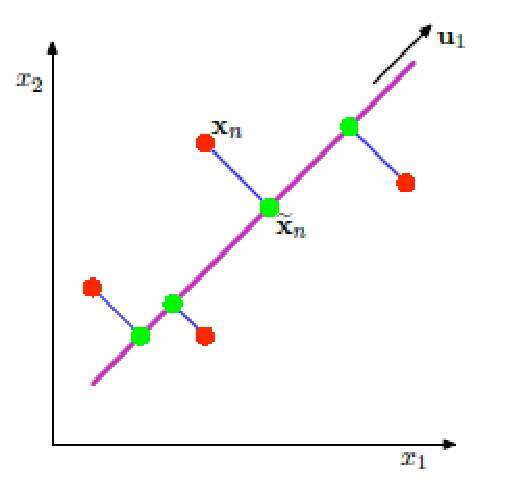
\includegraphics[width=0.4\linewidth]{figure/fig28.pdf}
\end{center}

\paragraph{Setting Up the Problem}

Let $\mathbf{u}_1$ be a unit vector ($\|\mathbf{u}_1\| = 1$) specifying the direction of the line along which we will project. Any point lying on the line passing through the mean $\mathbf{m}$ can be parameterized as:
\begin{myequation}
\mathbf{x} = \alpha\mathbf{u}_1 + \mathbf{m}
\end{myequation}
where $\alpha \in \mathbb{R}$ represents the signed distance from $\mathbf{m}$ along the direction $\mathbf{u}_1$. For each data point $\mathbf{x}_i$ (for $i = 1, \ldots, n$), its orthogonal projection onto this line is:
\begin{myequation}
\tilde{\mathbf{x}}_i = \alpha_i\mathbf{u}_1 + \mathbf{m}
\end{myequation}
for some scalar $\alpha_i$ that we must determine.

Our goal is to find both the optimal projection coefficients $\{\alpha_i\}_{i=1}^n$ for each data point and the optimal direction $\mathbf{u}_1$ for the line itself. Together, these should minimize the total reconstruction error—the sum of squared distances between original points and their projections:
\begin{myequation}
J(\alpha_1, \ldots, \alpha_n, \mathbf{u}_1) = \sum_{i=1}^{n}\|\tilde{\mathbf{x}}_i - \mathbf{x}_i\|^2 = \sum_{i=1}^{n}\|(\mathbf{m} + \alpha_i\mathbf{u}_1) - \mathbf{x}_i\|^2
\end{myequation}

This is a joint optimization problem over the continuous variables $\{\alpha_i\}$ and the unit vector $\mathbf{u}_1$. We will solve it in two stages: first optimizing the projection coefficients for a fixed direction, then optimizing the direction given the optimal coefficients.

\paragraph{Optimizing Projection Coefficients}

For a fixed direction $\mathbf{u}_1$, what are the optimal projection coefficients? Rearranging the objective and using the fact that data has been centered (we can work with $\mathbf{x}_i - \mathbf{m}$ in place of $\mathbf{x}_i$):
\begin{myequation}
J(\alpha_1, \ldots, \alpha_n, \mathbf{u}_1) = \sum_{i=1}^{n}\|\alpha_i\mathbf{u}_1 - (\mathbf{x}_i - \mathbf{m})\|^2
\end{myequation}

Expanding this using $\|\mathbf{a} - \mathbf{b}\|^2 = \|\mathbf{a}\|^2 + \|\mathbf{b}\|^2 - 2\mathbf{a}^T\mathbf{b}$ and noting that $\|\mathbf{u}_1\|^2 = 1$:
\begin{myequation}
J = \sum_{i=1}^{n}\alpha_i^2 + \sum_{i=1}^{n}\|\mathbf{x}_i - \mathbf{m}\|^2 - 2\sum_{i=1}^{n}\alpha_i\mathbf{u}_1^T(\mathbf{x}_i - \mathbf{m})
\end{myequation}

To minimize with respect to each $\alpha_k$, we compute the partial derivative:
\begin{myequation}
\frac{\partial J}{\partial \alpha_k} = 2\alpha_k - 2\mathbf{u}_1^T(\mathbf{x}_k - \mathbf{m})
\end{myequation}

Setting this equal to zero and solving yields:
\begin{myequation}
\alpha_k = \mathbf{u}_1^T(\mathbf{x}_k - \mathbf{m})
\end{myequation}

This is precisely the orthogonal projection of the centered data point $\mathbf{x}_k - \mathbf{m}$ onto the direction $\mathbf{u}_1$—exactly what geometric intuition suggests. The second derivative $\frac{\partial^2 J}{\partial \alpha_k^2} = 2 > 0$ confirms this is indeed a minimum rather than a maximum or saddle point.

\paragraph{Finding the Optimal Direction}

Having determined that the optimal projection coefficients are given by $\alpha_i = \mathbf{u}_1^T(\mathbf{x}_i - \mathbf{m})$, we now substitute these back into the objective function to obtain a function of $\mathbf{u}_1$ alone:
\begin{myequation}
J(\mathbf{u}_1) = \sum_{i=1}^{n}\alpha_i^2 + \sum_{i=1}^{n}\|\mathbf{x}_i - \mathbf{m}\|^2 - 2\sum_{i=1}^{n}\alpha_i^2
\end{myequation}

The second and third terms combine:
\begin{myequation}
J(\mathbf{u}_1) = -\sum_{i=1}^{n}\alpha_i^2 + \sum_{i=1}^{n}\|\mathbf{x}_i - \mathbf{m}\|^2
\end{myequation}

Substituting the expression for $\alpha_i$:
\begin{myequation}
J(\mathbf{u}_1) = -\sum_{i=1}^{n}[\mathbf{u}_1^T(\mathbf{x}_i - \mathbf{m})]^2 + \sum_{i=1}^{n}\|\mathbf{x}_i - \mathbf{m}\|^2
\end{myequation}

Now we introduce the sample covariance matrix, which will play a central role throughout PCA:
\begin{myequation}
\mathbf{S} = \frac{1}{n}\sum_{i=1}^{n}(\mathbf{x}_i - \mathbf{m})(\mathbf{x}_i - \mathbf{m})^T
\end{myequation}

To connect our objective to this matrix, observe that the scalar $[\mathbf{u}_1^T(\mathbf{x}_i - \mathbf{m})]^2$ can be rewritten using the identity $(a)(a)^T = a^2$ for scalars (here $a = \mathbf{u}_1^T(\mathbf{x}_i - \mathbf{m})$):
\begin{myequation}
[\mathbf{u}_1^T(\mathbf{x}_i - \mathbf{m})]^2 = \mathbf{u}_1^T(\mathbf{x}_i - \mathbf{m})(\mathbf{x}_i - \mathbf{m})^T\mathbf{u}_1
\end{myequation}

Summing over all data points:
\begin{myequation}
\sum_{i=1}^{n}\mathbf{u}_1^T(\mathbf{x}_i - \mathbf{m})(\mathbf{x}_i - \mathbf{m})^T\mathbf{u}_1 = \mathbf{u}_1^T\left[\sum_{i=1}^{n}(\mathbf{x}_i - \mathbf{m})(\mathbf{x}_i - \mathbf{m})^T\right]\mathbf{u}_1 = n\mathbf{u}_1^T\mathbf{S}\mathbf{u}_1
\end{myequation}

Therefore, the reconstruction error becomes:
\begin{myequation}
J(\mathbf{u}_1) = -n\mathbf{u}_1^T\mathbf{S}\mathbf{u}_1 + \sum_{i=1}^{n}\|\mathbf{x}_i - \mathbf{m}\|^2
\end{myequation}

\paragraph{Geometric Interpretation and the Variance Perspective}

The term $\mathbf{u}_1^T\mathbf{S}\mathbf{u}_1$ appearing in our objective has a natural and important interpretation: it represents the variance of the projected data along direction $\mathbf{u}_1$. To see why, recall that:
\begin{itemize}
\item $\alpha_i = \mathbf{u}_1^T(\mathbf{x}_i - \mathbf{m})$ is the projection of centered point $\mathbf{x}_i - \mathbf{m}$ onto $\mathbf{u}_1$
\item $\alpha_i^2 = [\mathbf{u}_1^T(\mathbf{x}_i - \mathbf{m})]^2$ is the squared value of this projection
\item $\frac{1}{n}\sum_{i=1}^{n}\alpha_i^2 = \frac{1}{n}\sum_{i=1}^{n}[\mathbf{u}_1^T(\mathbf{x}_i - \mathbf{m})]^2 = \mathbf{u}_1^T\mathbf{S}\mathbf{u}_1$ is the sample variance of these projected values (since the projected data is already centered)
\end{itemize}

Since the second term in $J(\mathbf{u}_1)$ is constant with respect to $\mathbf{u}_1$, minimizing the reconstruction error is equivalent to maximizing the variance of the projected data:
\begin{myequation}
\min{\|\mathbf{u}_1\|=1} J(\mathbf{u}_1) \quad \Leftrightarrow \quad \max_{\|\mathbf{u}_1\|=1} \mathbf{u}_1^T\mathbf{S}\mathbf{u}_1
\end{myequation}

This reveals a beautiful duality at the heart of PCA: minimizing reconstruction error is equivalent to maximizing variance in the projected space. This makes intuitive geometric sense. If we project data onto a direction of low variance, we are collapsing points that were far apart in the original space onto nearby points in the projected space, losing information and incurring large reconstruction errors. Conversely, projecting onto a direction of high variance preserves the spread of the data, maintaining distances and minimizing reconstruction error.

\paragraph{The Eigenvalue Solution}

The constrained optimization problem $\max_{\|\mathbf{u}_1\|=1} \mathbf{u}_1^T\mathbf{S}\mathbf{u}_1$ has a well-known solution from linear algebra. Using the method of Lagrange multipliers, we introduce a multiplier $\lambda_1$ for the constraint $\|\mathbf{u}_1\|^2 = 1$ and form the Lagrangian:
\begin{myequation}
\mathcal{L}(\mathbf{u}_1, \lambda_1) = \mathbf{u}_1^T\mathbf{S}\mathbf{u}_1 - \lambda_1(\mathbf{u}_1^T\mathbf{u}_1 - 1)
\end{myequation}

Setting the gradient with respect to $\mathbf{u}_1$ equal to zero:
\begin{myequation}
\frac{\partial \mathcal{L}}{\partial \mathbf{u}_1} = 2\mathbf{S}\mathbf{u}_1 - 2\lambda_1\mathbf{u}_1 = \mathbf{0}
\end{myequation}

This simplifies to the eigenvalue equation:
\begin{myequation}
\mathbf{S}\mathbf{u}_1 = \lambda_1\mathbf{u}_1
\end{myequation}

Therefore, the optimal direction $\mathbf{u}_1$ must be an eigenvector of the covariance matrix $\mathbf{S}$, with eigenvalue $\lambda_1$. Moreover, the variance along this direction is:
\begin{myequation}
\mathbf{u}_1^T\mathbf{S}\mathbf{u}_1 = \mathbf{u}_1^T(\lambda_1\mathbf{u}_1) = \lambda_1\mathbf{u}_1^T\mathbf{u}_1 = \lambda_1
\end{myequation}

Since we wish to maximize variance, we should choose $\mathbf{u}_1$ to be the eigenvector corresponding to the largest eigenvalue of $\mathbf{S}$. This eigenvector is called the first principal component, and its eigenvalue tells us how much variance is explained by projecting onto this direction.

This elegant result—that PCA reduces to an eigenvalue problem—is both computationally convenient and geometrically illuminating. The eigendecomposition of $\mathbf{S}$ reveals the natural coordinate system for the data, with each eigenvector representing a direction of variation and each eigenvalue quantifying how much variation occurs along that direction.

\subsubsection*{PCA for Multiple Dimensions: The General Case}

The one-dimensional case establishes the fundamental ideas, but in practice we often wish to project onto a $d'$-dimensional subspace where $1 < d' < D$. The generalization follows naturally from the one-dimensional solution.

If we seek a $d'$-dimensional subspace, we need $d'$ orthonormal basis vectors $\mathbf{u}_1, \ldots, \mathbf{u}_{d'}$ that span this subspace. By analogy with the one-dimensional case, we might guess that these should be the eigenvectors of $\mathbf{S}$ corresponding to the $d'$ largest eigenvalues. This guess turns out to be correct, as can be shown through careful extension of the variance maximization argument or reconstruction error minimization.

More formally, we can construct these components sequentially. Having found the first principal component $\mathbf{u}_1$ (the eigenvector with largest eigenvalue), we seek a second direction $\mathbf{u}_2$ that is orthogonal to $\mathbf{u}_1$ (to avoid redundancy) and maximizes variance subject to this orthogonality constraint. The solution is the eigenvector corresponding to the second-largest eigenvalue. Continuing this process, the $k$-th principal component is the eigenvector with the $k$-th largest eigenvalue, constrained to be orthogonal to all previous components.

The total variance explained by the first $d'$ principal components is:
\begin{myequation}
\text{Variance explained} = \sum_{j=1}^{d'}\lambda_j
\end{myequation}
while the total variance in the original data is:
\begin{myequation}
\text{Total variance} = \sum_{j=1}^{D}\lambda_j = \text{trace}(\mathbf{S})
\end{myequation}

The proportion of variance explained, a commonly reported diagnostic, is thus:
\begin{myequation}
\text{Proportion of variance explained} = \frac{\sum_{j=1}^{d'}\lambda_j}{\sum_{j=1}^{D}\lambda_j}
\end{myequation}

This quantity helps us choose how many components to retain: we typically look for a "knee" or "elbow" in the scree plot (a plot of eigenvalues versus component index) or retain enough components to explain a desired proportion of variance (commonly $80\%$, $90\%$, or $95\%$).

The projection of a data point $\mathbf{x}$ onto the first $d'$ principal components is:
\begin{myequation}
\mathbf{z} = \mathbf{U}_{d'}^T(\mathbf{x} - \mathbf{m})
\end{myequation}
where $\mathbf{U}_{d'} = [\mathbf{u}_1, \ldots, \mathbf{u}_{d'}] \in \mathbb{R}^{D \times d'}$ is the matrix of the first $d'$ principal components. The reconstruction from this projection is:
\begin{myequation}
\tilde{\mathbf{x}} = \mathbf{U}_{d'}\mathbf{z} + \mathbf{m} = \mathbf{U}_{d'}\mathbf{U}_{d'}^T(\mathbf{x} - \mathbf{m}) + \mathbf{m}
\end{myequation}

This reconstruction formula shows that PCA projection and reconstruction can be viewed as a linear transformation followed by its pseudo-inverse, projecting onto the subspace spanned by the principal components.

\subsubsection*{Linear Discriminant Analysis}

While Principal Component Analysis is fundamentally an unsupervised method that ignores class labels and focuses solely on variance structure, Linear Discriminant Analysis (LDA) , which was introduced above and will be shortly reminded here, takes a supervised approach tailored specifically for classification tasks. LDA seeks projections that maximize the separation between classes while simultaneously minimizing the spread within each class. This dual objective makes LDA particularly effective when the goal is to find low-dimensional representations that preserve or enhance class discriminability.

For binary classification with two classes $C_1$ and $C_2$, LDA finds a direction $\mathbf{w}$ such that when we project the data onto this direction, the two class distributions are as separated as possible. To formalize "separation," we need to quantify both how far apart the class means are and how tightly clustered each class is around its mean.

Let $\mathbf{m}_1$ and $\mathbf{m}_2$ denote the mean vectors for classes $C_1$ and $C_2$ in the original $D$-dimensional space. After projecting onto the direction $\mathbf{w}$, the class means become scalars:
\begin{myequation}
m_1 = \mathbf{w}^T\mathbf{m}_1 \quad \text{and} \quad m_2 = \mathbf{w}^T\mathbf{m}_2
\end{myequation}

The distance between class means in the projected space is $|m_2 - m_1| = |\mathbf{w}^T(\mathbf{m}_2 - \mathbf{m}_1)|$. A good projection should make this distance large, pulling the class distributions apart.

However, maximizing the distance between class means alone is insufficient. We could trivially make this distance arbitrarily large by choosing $\mathbf{w}$ to be a scaled version of $(\mathbf{m}_2 - \mathbf{m}_1)$. What we need in addition is a constraint that prevents the within-class scatter from also growing unboundedly. We want tight, well-separated clusters—not overlapping clouds with distant means.

To quantify within-class scatter, we compute the variance of the projected data within each class. For class $C_i$, the within-class covariance matrix in the original space is:
\begin{myequation}
\mathbf{S}_i = \sum_{\mathbf{x} \in C_i}(\mathbf{x} - \mathbf{m}_i)(\mathbf{x} - \mathbf{m}_i)^T
\end{myequation}

After projection, the within-class variance becomes:
\begin{myequation}
s_i^2 = \mathbf{w}^T\mathbf{S}_i\mathbf{w}
\end{myequation}

We define the total within-class covariance matrix as $\mathbf{S}_W = \mathbf{S}_1 + \mathbf{S}_2$, pooling scatter from both classes. Similarly, we define the between-class covariance matrix as:
\begin{myequation}
\mathbf{S}_B = (\mathbf{m}_2 - \mathbf{m}_1)(\mathbf{m}_2 - \mathbf{m}_1)^T
\end{myequation}
which captures how far apart the class means are.

The Fisher criterion, which LDA maximizes, is the ratio of between-class scatter to within-class scatter:
\begin{myequation}
J(\mathbf{w}) = \frac{(m_2 - m_1)^2}{s_1^2 + s_2^2} = \frac{\mathbf{w}^T\mathbf{S}_B\mathbf{w}}{\mathbf{w}^T\mathbf{S}_W\mathbf{w}}
\end{myequation}

This criterion elegantly balances the competing objectives: the numerator rewards large between-class separation, while the denominator penalizes large within-class scatter. A direction that achieves both tight clusters and distant means will yield a large Fisher criterion.

\paragraph{Optimization}

To maximize $J(\mathbf{w})$, we set its gradient to zero. Using the quotient rule for the gradient of a ratio:
\begin{myequation}
\nabla_{\mathbf{w}} \frac{\mathbf{w}^T\mathbf{S}_B\mathbf{w}}{\mathbf{w}^T\mathbf{S}_W\mathbf{w}} = \mathbf{0}
\end{myequation}

Applying the quotient rule yields:
\begin{myequation}
(\mathbf{w}^T\mathbf{S}_B\mathbf{w})\mathbf{S}_W\mathbf{w} - (\mathbf{w}^T\mathbf{S}_W\mathbf{w})\mathbf{S}_B\mathbf{w} = \mathbf{0}
\end{myequation}
which can be rearranged to:
\begin{myequation}
(\mathbf{w}^T\mathbf{S}_B\mathbf{w})\mathbf{S}_W\mathbf{w} = (\mathbf{w}^T\mathbf{S}_W\mathbf{w})\mathbf{S}_B\mathbf{w}
\end{myequation}


%Now observe that $\mathbf{w}^T\mathbf{S}_B\mathbf{w}$ and $\mathbf{w}^T\mathbf{S}_W\mathbf{w}$ are both scalars, which we denote $c_B$ and $c_W$ respectively. Moreover, since $\mathbf{S}_B = (\mathbf{m}_2 - \mathbf{m}_1)(\mathbf{m}_2 - \mathbf{m}_1)^T$, we have:
%\begin{myequation}
%\mathbf{S}_B\mathbf{w} = (\mathbf{m}_2 - \mathbf{m}_1)(\mathbf{m}_2 - \mathbf{m}_1)^T\mathbf{w} = (\mathbf{m}_2 - \mathbf{m}_1) c_m
%\end{myequation}
%where $c_m = (\mathbf{m}_2 - \mathbf{m}_1)^T\mathbf{w}$ is another scalar.
%
%Substituting into the optimality condition:
%\begin{myequation}
%c_B\mathbf{S}_W\mathbf{w} = c_W(\mathbf{m}_2 - \mathbf{m}_1)c_m
%\end{myequation}
%
%Solving for $\mathbf{w}$:
%\begin{myequation}
%\mathbf{w} = \frac{c_W c_m}{c_B}\mathbf{S}_W^{-1}(\mathbf{m}_2 - \mathbf{m}_1)
%\end{myequation}

In a  few passages, and taking into account that we are only interested in the direction of $\mathbf{w}$, Fisher's linear discriminant solution can be obtained:
\begin{myequation}
\hat{\mathbf{w}} = \mathbf{S}_W^{-1}(\mathbf{m}_2 - \mathbf{m}_1) = (\mathbf{S}_1 + \mathbf{S}_2)^{-1}(\mathbf{m}_2 - \mathbf{m}_1)
\end{myequation}

This elegant result shows that the optimal direction is obtained by first computing the vector connecting the class means in the original space, then transforming it by the inverse of the pooled within-class covariance matrix. The inverse covariance accounts for the different scales and correlations among features, effectively "whitening" the space to give equal weight to all directions before measuring separation.

%\subsubsection*{Choosing the Classification Threshold}
%
%Having determined the projection direction $\hat{\mathbf{w}}$, we need to select a threshold $\tilde{y}$ for classification. A principled approach is based on probabilistic modeling of the projected data.
%
%We model the projected data for each class as Gaussian: $p(y|C_i) \sim \mathcal{N}(m_i, \sigma_i^2)$, where the parameters are estimated via maximum likelihood:
%\begin{myequation}
%m_i = \frac{1}{n_i}\sum_{\mathbf{x} \in C_i}\mathbf{w}^T\mathbf{x} \quad \text{and} \quad \sigma_i^2 = \frac{1}{n_i - 1}\sum_{\mathbf{x} \in C_i}(\mathbf{w}^T\mathbf{x} - m_i)^2
%\end{myequation}
%where $n_i$ is the number of training samples in class $C_i$.
%
%Applying Bayes' rule, we compute posterior probabilities:
%\begin{myequation}
%p(C_i|y) \propto p(y|C_i)p(C_i) = p(y|C_i)\frac{n_i}{n_1 + n_2} \propto n_i \exp\left(-\frac{(y - m_i)^2}{2\sigma_i^2}\right)
%\end{myequation}
%
%The decision threshold $\tilde{y}$ is the value where the class posteriors are equal. Equivalently, we choose $\tilde{y}$ as the smallest $y$ satisfying:
%\begin{myequation}
%\frac{p(C_2|y)}{p(C_1|y)} = \frac{n_2}{n_1}\frac{p(y|C_2)}{p(y|C_1)} > 1
%\end{myequation}
%
%This threshold balances the trade-off between false positives and false negatives, taking into account both the class-conditional distributions and the prior class probabilities (estimated from the training set class proportions).

\subsection*{Autoencoders}

While methods like PCA and LDA are constrained to learn linear projections, autoencoders harness the representational power of neural networks to discover nonlinear low-dimensional representations of high-dimensional data. An autoencoder learns to compress data into a compact latent representation through an encoding transformation, then reconstruct the original data from this compressed form through a decoding transformation. The requirement that the data be recoverable from its compressed representation ensures that the encoding captures the information essential for representing the data, while the dimensionality bottleneck forces the discovery of efficient, parsimonious representations.

Formally, an autoencoder for data in $\mathbb{R}^n$ with a latent representation in $\mathbb{R}^p$ (where typically $p \ll n$) can be defined in terms of three components. First, we have a class of encoder functions $\mathcal{E}$, consisting of parameterized mappings from $\mathbb{R}^n$ to $\mathbb{R}^p$. Second, we have a class of decoder functions $\mathcal{D}$, consisting of parameterized mappings from $\mathbb{R}^p$ back to $\mathbb{R}^n$. Third, we define a reconstruction loss function $\mathcal{L}: \mathbb{R}^n \times \mathbb{R}^n \to \mathbb{R}$ that quantifies how well the reconstructed output matches the original input.

The learning problem is to find a pair of encoder and decoder functions $e^* \in \mathcal{E}$ and $d^* \in \mathcal{D}$ that minimize the expected reconstruction loss:
\begin{myequation}
(e^*, d^*) = \argmin{e \in \mathcal{E}, d \in \mathcal{D}} \mathbb{E}_{\mathbf{x}}[\mathcal{L}(\mathbf{x}, d(e(\mathbf{x})))]
\end{myequation}

That is, we seek the encoder-decoder pair which minimizes the expected difference between the original input $\mathbf{x}$ and the result of the encoding-decoding sequence $d(e(\mathbf{x}))$. In practice, this expectation is approximated by averaging over the training set. The reconstruction loss is typically chosen to be the squared $\ell_2$ norm, $\mathcal{L}(\mathbf{x}, \mathbf{y}) = \|\mathbf{x} - \mathbf{y}\|^2 = \sum_{i=1}^n (x_i - y_i)^2$, though other choices such as cross-entropy are appropriate for binary or categorical data.

Figure~\ref{fig:Autoencoder} provides a schematic illustration of the autoencoder architecture. The input $\mathbf{x}$ passes through the encoder $e$, yielding a compressed latent representation $\mathbf{z} = e(\mathbf{x})$. This latent vector then passes through the decoder $d$, producing a reconstruction $\mathbf{y} = d(\mathbf{z}) = d(e(\mathbf{x}))$. The training objective is to minimize the discrepancy between $\mathbf{x}$ and $\mathbf{y}$ across the training dataset.

\begin{figure}
\begin{center}
\begin{tikzpicture}
\Vertex[Math, x=0, y=0, color=xkcdTurquoise, opacity=.5, shape = rectangle, fontsize=\footnotesize, style={minimum width=.3cm, minimum height=2.5cm, line width=.1pt}]{B1}
\Text[x=0,y=1.5, distance=7mm, fontsize=\footnotesize]{$\x$}
\Text[position=left, x=0,y=.5, distance=2mm, fontsize=\scriptsize]{$n$}

\Vertex[Math, x=1.5,y=0, color=xkcdBuff, label = e, size = 1, opacity=.5, fontsize=\large, style={line width=.5pt}]{C}
 \Edge[lw=.5pt, Direct](B1)(C)
 
\Vertex[Math, x=3, y=0, color=xkcdLipstickRed, opacity=.5, shape = rectangle, fontsize=\footnotesize, style={minimum width=.3cm, minimum height=1.5cm, line width=.1pt}]{B2}
\Text[x=3,y=1.5, distance=7mm, fontsize=\footnotesize]{$\z=e(\x)$}
\Text[position=left, x=3,y=.5, distance=2mm, fontsize=\scriptsize]{$p$}

 \Edge[lw=.5pt, Direct](C)(B2)
 
 \Vertex[Math, x=4.5,y=0, color=xkcdBurntOrange, label = d, size = 1, opacity=.5, fontsize=\large, style={line width=.5pt}]{C1}
 \Edge[lw=.5pt, Direct](B2)(C1)
 
 \Vertex[Math, x=6, y=0, color=xkcdFadedBlue, opacity=.5, shape = rectangle, fontsize=\footnotesize, style={minimum width=.3cm, minimum height=2.5cm, line width=.1pt}]{B3}
 \Text[x=6,y=1.5, distance=7mm, fontsize=\footnotesize]{$\y=d(\z)$}
\Text[position=right, x=6,y=.5, distance=2mm, fontsize=\scriptsize]{$n$}
 \Edge[lw=.5pt, Direct](C1)(B3)
 
  \Edge[lw=.5pt, bend=90, label=loss, fontsize=\small, style={dashed,color=xkcdRed}](B1)(B3)
\end{tikzpicture}
\end{center}
\caption{General structure of an autoencoder.}%
\label{fig:Autoencoder}
\end{figure}

Starting from the input $\mathbf{x}$, the encoder derives a new vector $\mathbf{z}$ of different (usually smaller) dimensionality. This compressed vector is called a latent representation of $\mathbf{x}$, and it forms the low-dimensional embedding we seek. In the most popular form of autoencoders, both the encoder $e$ and decoder $d$ are implemented as neural networks, which allows them to learn complex nonlinear transformations that would be impossible with linear methods.

An interesting special case arises when we restrict $\mathcal{E}$ and $\mathcal{D}$ to be classes of linear operations. In this case, each component of $\mathbf{z}$ is a linear combination of components of $\mathbf{x}$, and each component of $\mathbf{y}$ is a linear combination of components of $\mathbf{z}$. Under these constraints, the linear autoencoder recovers the same latent representation as Principal Component Analysis, establishing a deep connection between the two approaches. Therefore, an autoencoder can be viewed as a generalization of PCA. Where PCA finds a low-dimensional hyperplane in which the data approximately lies, the autoencoder can learn a nonlinear manifold. Moreover, unlike PCA which focuses solely on variance, the autoencoder is explicitly optimized for data reconstruction from the compressed code, which may better preserve task-relevant information.

\begin{figure}
\begin{center}
\resizebox{0.8\textwidth}{!}{%
\begin{tikzpicture}[
    shorten >=1pt, shorten <=1pt, >=stealth',
    neuron/.style={circle, draw, minimum size=4ex, thick, fill=#1, opacity=0.7},
    legend/.style={font=\large\bfseries},
  ]

  % encoder
  \drawNodes{encoder}{{{,,,,,}, {,,,,}, {,,,,}}}{xkcdTeal}
  \denselyConnectNodes{encoder}{{6, 5, 5}}

  % decoder
  \begin{scope}[xshift=7cm]
    \drawNodes{decoder}{{{,,,}, {,,,,,}}}{xkcdBuff}
    \denselyConnectNodes{decoder}{{4, 6}}
  \end{scope}

  % mu, sigma, sample nodes
  \foreach \idx in {1,...,3} {
      \coordinate[neuron, right=1 of encoder-3-3, yshift=\idx cm-2cm, fill=xkcdFadedBlue, fill opacity=0.7] (latent-\idx);
    }

 % mu, sigma, sample boxes
 \node [label=latent, fit=(latent-1) (latent-3), draw, fill=xkcdFadedBlue, opacity=0.2] (latent) {};
 \node [label=Encoder, fit=(encoder-1-1) (encoder-3-5) (encoder-1-6), draw, fill=xkcdTurquoise, opacity=0.2] (encoder) {};
 \node [label=Decoder, fit=(decoder-1-1) (decoder-2-1) (decoder-2-6), draw, fill=xkcdBuff, opacity=0.2] (decoder) {};
   
  % mu, sigma, sample connections
 % \draw[->] (mu.east) edge (sample.west) (sigma.east) -- (sample.west);
  \foreach \a in {1,2,3,4,5}
  \foreach \b in {1,2,3} {
      \draw[->] (encoder-3-\a) -- (latent-\b);
    }
    
  \foreach \a in {1,2,3,4}
  \foreach \b in {1,2,3} {
      \draw[->] (latent-\b) -- (decoder-1-\a);
    }

  % input + output labels
  \foreach \idx in {1,...,6} {
      \node[left=0.2 of encoder-1-\idx] {$x_\idx$};
      \node[right=0.2 of decoder-2-\idx] {$\hat x_\idx$};
    }
  \node[above left=0.5 of encoder-1-4] {input};
  \node[above right=0.5 of decoder-2-4] {output};

\end{tikzpicture}
    }%
\end{center}
\caption{Neural network implementation of an autoencoder.}%
\label{fig:Autoencoder_nn}
    %\label{fig:var_encoder}
\end{figure}


In practice, the encoder and decoder are parameterized as classes of functions with learnable parameters. The encoder is characterized by parameters $\boldsymbol{\theta}$ and the decoder by parameters $\boldsymbol{\phi}$. The loss function is then minimized with respect to these parameters:
\begin{myequation}
(\boldsymbol{\theta}^*, \boldsymbol{\phi}^*) = \argmin{\boldsymbol{\theta}, \boldsymbol{\phi}} \mathbb{E}_{\mathbf{x}}[\mathcal{L}(\mathbf{x}, d(e(\mathbf{x}; \boldsymbol{\theta}); \boldsymbol{\phi}))]
\end{myequation}

These parametric functions are typically implemented as neural networks, trained via backpropagation and stochastic gradient descent. Figure~\ref{fig:Autoencoder_nn} illustrates a concrete neural network instantiation of an autoencoder, showing the layered structure of the encoder (which progressively compresses the representation) and the decoder (which progressively expands it back to the original dimensionality).

Figure~\ref{fig:lin_autoencoder} depicts the structure of a linear autoencoder in detail, showing the weight matrices $\mathbf{W}_e$ and $\mathbf{W}_d$ for the encoder and decoder, along with bias terms. The forward pass computes $\mathbf{z} = \mathbf{W}_e^T\mathbf{x} + \mathbf{b}$ (encoding) followed by $\mathbf{y} = \mathbf{W}_d^T\mathbf{z} + \mathbf{b}'$ (decoding), with the reconstruction loss measured between $\mathbf{x}$ and $\mathbf{y}$.

\begin{figure}
\begin{center}
\begin{tikzpicture}
\Vertex[Math, x=1.25,y=0, color=xkcdTurquoise, opacity=.8, shape = rectangle, label = \x, fontsize=\footnotesize, style={minimum width=2cm, minimum height=3mm, line width=.1pt}]{B0}
  \Text[position=below,x=1.25,y=0, distance=1.2mm, fontsize=\scriptsize]{$n$}
  \Vertex[Math, x=3.5,y=0, color=xkcdBuff, opacity=.5, shape = rectangle, label = W_e, fontsize=\footnotesize, style={minimum width=1cm, minimum height=2cm, line width=.5pt}]{W1}
  \Text[position=above,x=3.5,y=0, distance=11mm, fontsize=\scriptsize]{$p$}
  \Text[position=right,x=3.5,y=.5, distance=6mm, fontsize=\scriptsize]{$n$}
  \Edge[lw=.5pt, Direct](B0)(W1)
  
  \Vertex[Math, x=4.75,y=0, color=xkcdLightGrey, label = +, size = .4, opacity=.5, fontsize=\footnotesize, style={line width=.5pt}]{C}
  \Edge[lw=.5pt, Direct](W1)(C)
  
\Vertex[Math, x=4.75,y=-1, color=xkcdBuff, label = b, opacity=.5, shape = rectangle, fontsize=\footnotesize, style={minimum width=9mm, minimum height=3mm, line width=.5pt}]{B3}
\Text[position=below,x=4.75,y=-1, distance=2mm, fontsize=\scriptsize]{$p$}
\Edge[lw=.5pt, Direct](B3)(C)
    
\Vertex[Math, x=6,y=0, color=xkcdLipstickRed, label=\z, opacity=.5, shape = rectangle, fontsize=\footnotesize, style={minimum width=1cm, minimum height=3mm, line width=.1pt}]{B2}
 \Text[position=below,x=6,y=0, distance=2mm, fontsize=\scriptsize]{$p$}
 \Edge[lw=.5pt, Direct](C)(B2)
  
\Vertex[Math, x=8,y=0, color=xkcdBurntOrange, opacity=.5, shape = rectangle, label = W_d, fontsize=\footnotesize, style={minimum width=2cm, minimum height=1cm, line width=.5pt}]{B4}
  \Text[position=above,x=8,y=0, distance=6mm, fontsize=\scriptsize]{$n$}
  \Text[position=right,x=8.5,y=.25, distance=5mm, fontsize=\scriptsize]{$p$}
\Edge[lw=.5pt, Direct](C1)(B2)
\Edge[lw=.5pt, Direct](B2)(B4)
  
\Vertex[Math, x=10,y=0, color=xkcdLightGrey, label = +, size = .4, opacity=.5, fontsize=\footnotesize, style={line width=.5pt}]{C2}
\Edge[lw=.5pt, Direct](B4)(C2)
  
\Vertex[Math, x=10,y=-1, color=xkcdBurntOrange, label = b', opacity=.5, shape = rectangle, fontsize=\footnotesize, style={minimum width=2cm, minimum height=3mm, line width=.5pt}]{B5}
\Text[position=below,x=10,y=-1, distance=2mm, fontsize=\scriptsize]{$n$}
\Edge[lw=.5pt, Direct](B5)(C2)
    
 \Vertex[Math, x=12,y=0, color=xkcdFadedBlue, label=\y, opacity=.5, shape = rectangle, fontsize=\footnotesize, style={minimum width=2cm, minimum height=3mm, line width=.1pt}]{C6}
 \Text[position=below,x=12,y=0, distance=2mm, fontsize=\scriptsize]{$n$}
\Edge[lw=.5pt, Direct](C2)(C6)
  \Edge[lw=.5pt, bend=90, label=loss, fontsize=\small, style={dashed,color=xkcdRed}](B0)(C6)
\end{tikzpicture}
\end{center}
\caption{Structure of a linear autoencoder.}%
\label{fig:lin_autoencoder}
\end{figure}

The concept of a "bottleneck" is central to the autoencoder's ability to learn useful representations. By making the latent feature's dimensionality $p$ lower (often much lower) than the input dimensionality $n$, we force the autoencoder to discover a compressed representation that captures the essential structure of the data while discarding noise and redundancy. This bottleneck ensures that the autoencoder cannot simply learn the identity function—it must learn to abstract and compress.

However, achieving meaningful compression requires more than just a dimensional bottleneck. Without additional constraints or regularization, an autoencoder with sufficient capacity in its encoder and decoder networks could memorize the training data, learning to map each training example to a unique index in the latent space and storing a lookup table for reconstruction. To prevent such trivial solutions and encourage the discovery of genuinely useful representations, several regularization strategies have been developed.

The most straightforward regularization is architectural: making the bottleneck dimensionality smaller than the input forces compression. However, even with a single-node bottleneck, overfitting remains possible if the encoder and decoder networks are complex enough to implement arbitrary mappings. More sophisticated regularization approaches include denoising autoencoders, which train the network to reconstruct clean inputs from corrupted versions, forcing it to learn robust features that capture the underlying structure rather than superficial details. Sparse autoencoders add penalties that encourage the latent representation to have many zero or near-zero components, promoting discovery of independent features. Variational autoencoders impose probabilistic structure on the latent space, ensuring that it has desirable properties for generation and interpolation.

In cases where the size of the hidden layer is equal to or greater than the size of the input, preventing the autoencoder from learning the identity function becomes particularly important. Several regularization options exist to enforce meaningful learning without creating a strict dimensional bottleneck, including the denoising and sparsity approaches mentioned above, as well as contractive autoencoders that penalize sensitivity of the representation to small input perturbations.

